
\chapter{Developing web applications}
web applications are on the rise. Not a day goes by where a new
web application isn't popping up for uses that were previously reserved for a
program locally installed on a computer. Even more so: Previously
unimagined uses for any Internet enabled device seem to be developed
at a rate that surpasses the former.

\section{What are web applications?}
Any web application can be divided into a server part and a client part.
Mostly both parts play a role in providing functionality to a web application.
The server holds persistent data in order for the user to be able to connect
from any machine. Since the server is not in the same location as the
client machine, latency in responses to user actions are a problem.
This problem is solved by letting the client part of the web application compute
responses where information on the server is not required. Queries to the server
can happen both synchronously and asynchronously, meaning a function can either
wait for the server response and block further execution of code until the
response is available or it can define a callback function which is invoked
once the response is available.

\begin{figure}
	\centering
	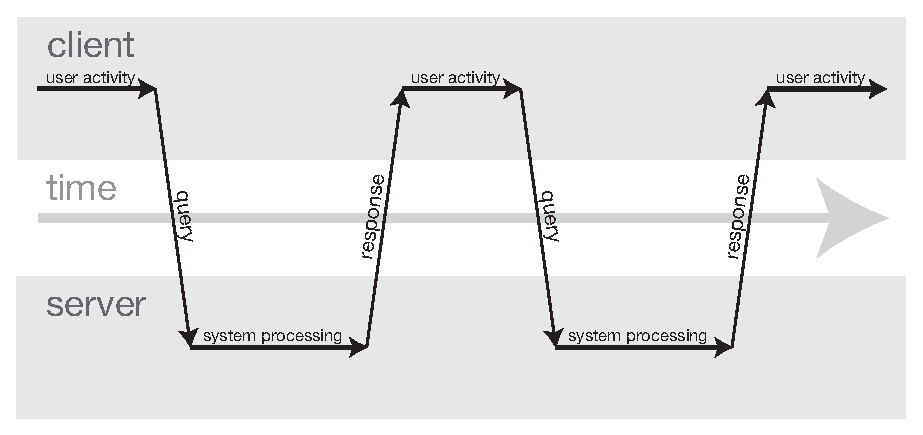
\includegraphics{graphics/synchronous}
	\caption{Diagram of synchronous communication between client and server}
\end{figure}

In this thesis, we will focus on web applications which use a
modern web browser and with it HTML as their basis (HTML5 in particular).
The non-static parts, which control the heart of the web application,
are supplied by JavaScript. This not only includes interactivity, but also
animation and updates from the server.\\
Interactivity in this context is defined as anything in the web application
the user can modify directly via an input device or modify indirectly, e.g.,
the back button in the browser and the window size of the browser.

Alternatives to JavaScript like Dart, CoffeeScript and Google Web Toolkit
do exist and are meant to ameliorate the shortcomings of JavaScript. 
However, they are all translated into JavaScript if cross-browser
compatibility is a requirement (which it almost always is).

The claim that web applications are meant to be ubiquitous,
operating system independent and run in the browser, is not a claim shared
by all definitions of a web application. For simplicity however we will for the
remainder of this thesis treat it as fact.

\subsection{Server side web applications}
Another way to incorporate business logic \todo{definition} and
interactivity into a web application, is by rendering customized HTML pages
on the server.\\
This has both advantages and disadvantages to the client-side scripting method:
\begin{itemize}
	\item \emph{Heavy computations can be run in a controllable time frame
	regardless of the client device.}\\
		Especially phones and other portable devices have reduced computing
		capacity in order to save battery power.
	\item \emph{Sensitive data can be handled without leaking it to the
	client.}\\
		Any data that the client is not supposed to see, can never leave the
		server. This means if any computation on the data should take place,
		it would have to be made insensitive, e.g., in the case of personal data
		for statistical purposes, the data would have to be anonymized first.
	\item \emph{The client application has to be initialized with data for each
	page load.}\\
		Data that gives the application context, is -- depending on the language
		and implementation -- loaded in RAM and/or saved in a database. On the
		client this data would first have to be loaded either from the server or
		from the local storage.
	\item \emph{The technology stack is more controllable.}\\
		The main browser technology stack, i.e., CSS, HTML and JavaScript,
		has suffered greatly under the "browser wars" \todo{reference}
		and has only gained widespread standardization in the last 5 years.
		There are still many inconsistencies, especially when tackling edge cases
		(for example the "Guillotine bug" in Microsoft Internet Explorer 6 and 7,
		each with their own variation
		\todo{http://www.positioniseverything.net/explorer/guillotine.html}).
		This technology stack and its edge cases is greatly reduced when
		on the server, because every software version and the software itself can
		be controlled by the developer.
\end{itemize}

\subsection{Client side web applications}

These arguments do not make the case for a server-only web application.
They highlight the strengths of server side processing. A combination of
server-side and client-side processing where their respective advantages
are utilized and their drawbacks avoided, would in part help in creating
an optimal web application.

\todo{Explain why client side programming advantages are obvious.
The above is mainly done to draw lines in the sand, between client
and server side.}

\begin{figure}
	\centering
	% !TEX root = ../thesis.tex
\newcommand{\drawheight}{6}
\newcommand{\boxheight}{\drawheight/3}
\newcommand{\lnlength}{\textwidth/7}
\newcommand{\commlength}{\textwidth/7/4}
\tikzset{corners/.style={fit={#1},rectangle,inner sep=0}}
\begin{tikzpicture}
	\node[fill=lgray,
		corners={(0,0) (\textwidth,\boxheight)}]
		(serverbg) {};
	\node[below=0.0 of serverbg.north] {\sffamily\huge\color{gray}{server}};
	
	\node[fill=lgray,draw=lgray,
		corners={(0,\boxheight*2) (\textwidth,\drawheight)}]
		(clientbg) {};
	\node[above=0.0 of clientbg.south] {\sffamily\huge\color{gray}{client}};
	
	\node[corners={(0,\boxheight) (\textwidth,\boxheight*2)}]
		(timebg) {};
	\node[below=0.0 of clientbg.south west,anchor=north west] {\sffamily\huge\color{gray}{time}};
	
	
	\draw[->,fill=lgray,draw=lgray,line width=5pt]
		let \p1 = (timebg.west) in (0,\y1) -- (\textwidth,\y1);
	
	
	\draw[->,line width=2pt]
		let \p1 = (clientbg.west) in
			(\x1,\y1) node (C1) {}
		--
			(\lnlength,\y1) node[pos=0.5,above]{user activity} node (C1') {};
	
	\draw[->,line width=2pt]
		let \p1 = (clientbg) in
			(\x1-\lnlength/2,\y1) node (C2) {}
		--
			(\x1+\lnlength/2,\y1) node[pos=0.5,above]{user activity} node (C2') {};
	
	\draw[->,line width=2pt]
		let \p1 = (clientbg.east) in
			(\x1-\lnlength,\y1) node (C3) {}
		--
			(\x1,\y1) node[pos=0.5,above]{user activity} node (C3') {};
	
	
	
	\draw[->,line width=2pt]
		let \p1 = (serverbg), \p2 = (C1'), \p3 = (C2) in
			(\x2+\commlength,\y1) node (S1) {}
				--
			(\x3-\commlength,\y1) node[pos=0.5,below]{server processing} node (S1') {};
	
	
	\draw[->,line width=2pt]
		let \p1 = (serverbg), \p2 = (C2'), \p3 = (C3) in
			(\x2+\commlength,\y1) node (S2) {}
		--
			(\x3-\commlength,\y1) node[pos=0.5,below]{server processing} node (S2') {};
	
		
	\draw[->] (C1') -- (S1) node[pos=0.5,above,sloped] {query};
	\draw[->] (S1') -- (C2) node[pos=0.5,above,sloped] {response};
	\draw[->] (C2') -- (S2) node[pos=0.5,above,sloped] {query};
	\draw[->] (S2') -- (C3) node[pos=0.5,above,sloped] {response};
	
	\draw[->,dashed] (C1') -- (C2) node[pos=0.5,above] {user activity};
	\draw[->,dashed] (C2') -- (C3) node[pos=0.5,above] {user activity};
\end{tikzpicture}

	\caption{Diagram of asynchronous communication between client and server}
\end{figure}

\section{The development process}
The development process of a web application is similar to any other
software development process. One starts with the data to be modeled.
It may be developed for the client and server part simultaneously.
A protocol for communication between the two is then established.
The design of a web application is usually the last component to fall
into place. It may have existed in the very beginning of the development
process, but is usually only finished and implemented when most other critical
components are in place.

\subsection{Usual design patterns}
Design patterns help developers to organize software projects into agreed upon
components, where each component has a specific function
(also referred to as "concerns" or "responsibility").
Although their exact features may not be known when a developer is first
introduced to a new software project, design patterns help him to quickly
recognize where functionality may be located in the code.

Instead of requiring developers to think up new structures, Design patterns
also help developers with grouping new code into well known components.

We will focus on one specific design pattern in this thesis. There many others,
which are relevant in web application development. There is nonetheless one
prevalent design pattern which we will examine in the following.

\subsubsection{Model-View-Controller}
The Model-View-Controller design pattern has proven itself to be a sane
choice for developing web applications. Most frameworks today use this
pattern or variations thereof.
It lends itself very well to web applications because of the client server
model, components of this pattern can be present on both sides allowing the
structure to be homogeneous.

\begin{itemize}
	\item The "Model" part represents the "data". All dynamic parts of an
	application modify, create or delete data, however ephemeral this data may
	be. Since much of the data can grouped, because it belongs to the same
	entity, it makes sense to represent those entities in the code and
	attach the data to them. This constitutes a Model. Besides this data,
	the Model can also have functions attached to it, which can act upon the data
	in various ways.
	\item A "Controller" implements the business logic that is decoupled from one
	specific Model. It draws on the functions tied to the models to perform its
	duties. Both of these components may be present on the server as well
	as the client.
	\item This is true for the "View" component as well. Its purpose however only
	comes to fruition on the client. This component is present on both the server
	and the client. Any HTML the server sends to the client is considered part of
	the "View" component.\\
	The job of the "View" component is to present the data to the user and
	tie calls to the controller to elements of the interface that can be acted
	upon by the user.
\end{itemize}

Designs of web applications change with time, features are added or
removed and common processes simplified. In light of this, it is
desirable to ensure that the "View" part of the Model-View-Controller
pattern is easily modifiable.

Modifications of this pattern have evolved in the web application domain to
cater to this specific purpose. The most notable of those would be the
Model-View-ViewModel pattern. It was designed by Microsoft and targeted at
interface development platforms including Windows Presentation Foundation and
Silverlight but also HTML5.\todo{reference}

The "ViewModel" component allows developers to implement interface logic that
lies between the Model and the View, allowing the view to be entirely free
of code. This component is meant to hold data-bindings to the Model while
listening to interface events at the same time. It "translates" user actions
into operations on the Model. Without it, the view would have to be aware of how
data is laid out internally, making refactoring of code harder.

The advantage of this version of Model-View-Controller is the improved
separation of responsibility between interface developers and application
developers. Neither will be required to modify or thoroughly understand the code
of the other. Even if both roles are filled by the same person,
separation of responsibility in an application still has its merits.

\todo{MVVM from Microsoft, MVP by Taligent (Apple, IBM, HP)}
